\documentclass[12pt]{article}
\usepackage{amsmath}
\usepackage{amssymb}
\usepackage[letterpaper,top=1.2in,bottom=1in,left=0.75in,right=0.75in,centering]{geometry}
%\usepackage{fancyhdr}
\usepackage{enumerate}
%\usepackage{lastpage}
\usepackage{multicol}
\usepackage{graphicx}

\reversemarginpar

%\pagestyle{fancy}
%\cfoot{}
%\lhead{Math 1560}\chead{Test \# 1}\rhead{May 18th, 2017}
%\rfoot{Total: 10 points}
%\chead{{\bf Name:}}
\newcommand{\points}[1]{\marginpar{\hspace{24pt}[#1]}}
\newcommand{\skipline}{\vspace{12pt}}
%\renewcommand{\headrulewidth}{0in}
\headheight 30pt

\newcommand{\di}{\displaystyle}
\newcommand{\abs}[1]{\lvert #1\rvert}
\newcommand{\len}[1]{\lVert #1\rVert}
\renewcommand{\i}{\mathbf{i}}
\renewcommand{\j}{\mathbf{j}}
\renewcommand{\k}{\mathbf{k}}
\newcommand{\R}{\mathbb{R}}
\newcommand{\aaa}{\mathbf{a}}
\newcommand{\bbb}{\mathbf{b}}
\newcommand{\ccc}{\mathbf{c}}
\newcommand{\dotp}{\boldsymbol{\cdot}}
\newcommand{\bbm}{\begin{bmatrix}}
\newcommand{\ebm}{\end{bmatrix}}                   
                  
\begin{document}


\author{Instructor: Sean Fitzpatrick}
\thispagestyle{empty}
\vglue1cm
\begin{center}
{\bf MATH 2565 - Tutorial \#11 Solutions}
\end{center}
\begin{multicols}{2}
\textbf{Extra fun:} A cow is tied to a silo or radius $R$ by a rope just long enough to reach the opposite side of the silo. Find the grazing area available to the cow.

\begin{center}
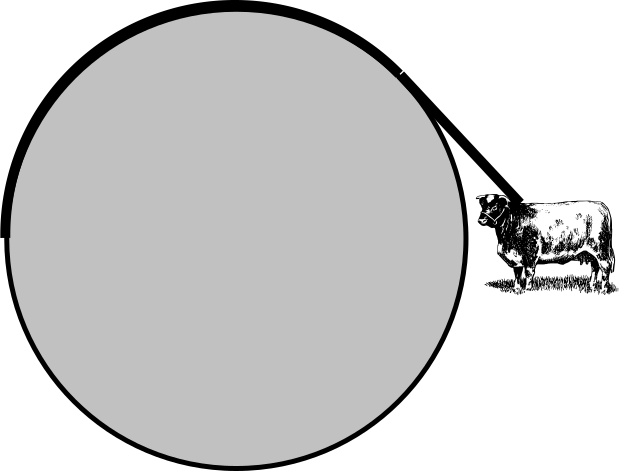
\includegraphics[width=0.9\columnwidth]{cowpic}
\end{center}
\end{multicols}

\textbf{Solution:} First, we need to determine the parametric equations for the path walked by the cow if she keeps the rope tight. (The resulting curve is part of the \textit{involute} of the circle.)

\begin{multicols}{2}
Referring to the diagram on the right, note that the angle at the top of the right-angled triangle through the points $(R\cos\theta,R\sin\theta)$ and the point $(x,y)$ we're looking for is also $\theta$. (This can be worked out using the fact that the angles of a triangle sum to $\pi$.)

The amount of rope unwound through an angle of $\theta$ is $R\theta$, so this is the length of the hypotenuse of our triangle.

\columnbreak

\begin{center}
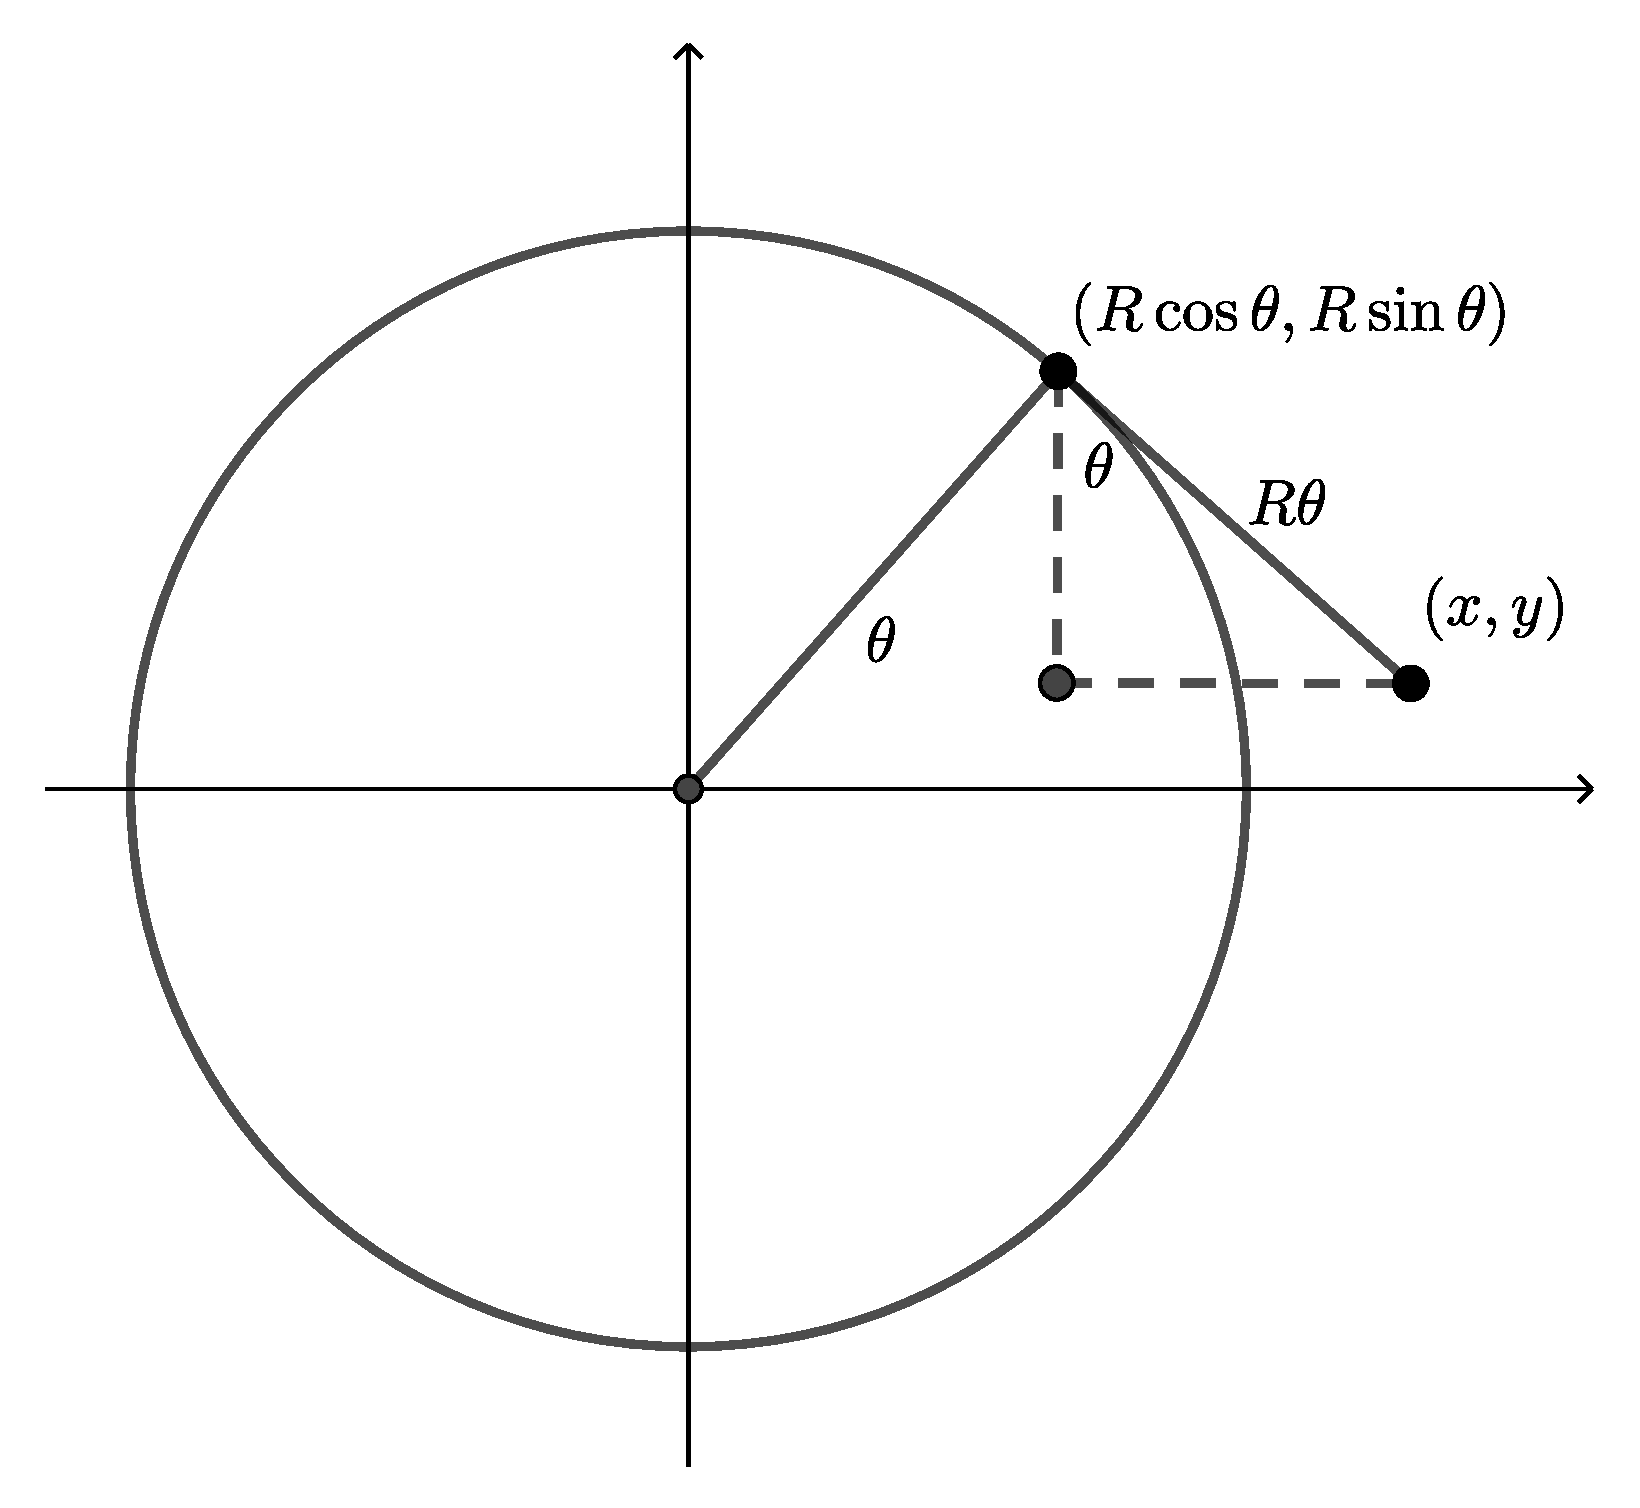
\includegraphics[width=\columnwidth]{cow-silo2}
\end{center}
\end{multicols}

The opposite side thus has length $(R\theta)\sin\theta$, and adding this to the $x$ value of the point on the circle, we find that the $x$ coordinate of the point we're looking for is therefore:
\[
x= R\cos\theta+R\theta\sin\theta=R(\cos\theta+\theta\sin\theta).
\]
Similarly, the $y$ coordinate is obtained by subtracting the length of the adjacent side from the $y$ value of the point on the circle, so
\[
y=R\sin\theta-R\theta\cos\theta = R(\sin\theta-\theta\cos\theta).
\]

\begin{multicols}{2}
Now, to compute the area, we need to realize that there are three parts to the boundary. First, the involute described above, for $0\leq \theta\leq \pi$. Once we reach $\theta=\pi$, we have used all the rope. If the cow continues towards the left, it traces out the left half of a circle of radius $\pi R$, centred at the point $(-R,0)$. Finally, once the cow reaches the bottom of the circle and continues below the silo, the rope begins to wrap around the bottom, and we trace out the same involute, for $-\pi\leq \theta\leq 0$.

By symmetry, it's enough to compute the top half of the area, and then double it. The total area is given by
\[
A = 2(A_1 -A_2 +A_3),
\]
where $A_1$ is the area under the involute, for $0\leq \theta\leq \pi$, $A_2$ is the area of half the silo, and $A_3$ is the area of a quarter circle of radius $\pi R$.
\columnbreak
\begin{center}
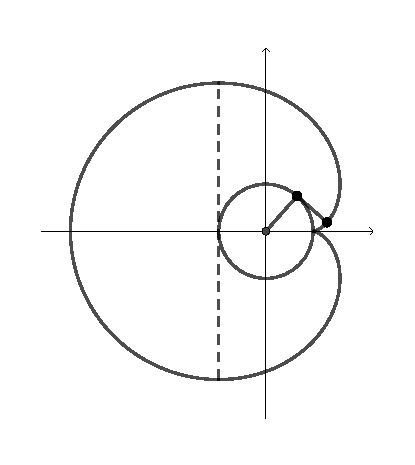
\includegraphics[width=\columnwidth]{cow-silo3}
\end{center}



\end{multicols}
 We immediately get:
\[
A_2 = \frac12 \pi R^2 \quad \text{ and } \quad A_3 = \frac14 \pi (\pi R)^2 = \frac14 \pi^3 R^2,
\]
while
\begin{align*}
A_1 &= -\int_0^{\pi}y(\theta)x'(\theta)\,d\theta\\
    &= -\int_0^{\pi} R(\sin\theta-\theta\cos\theta)\cdot R\theta\cos\theta\,d\theta\\
    &= -R^2\int_0^{\pi}(\theta\sin\theta\cos\theta-\theta^2\cos^2\theta)\,d\theta\\
    &=\frac{\pi R^2}{2}+\frac{\pi^3 R^2}{6}.
\end{align*}
The total area is therefore $A=\dfrac{\pi^3R^2}{3}+\dfrac{\pi^3R^2}{2}=\dfrac{5\pi^3R^2}{6}$. 
\newpage
%\thispagestyle{empty}





 \begin{enumerate}
\item Eliminate the parameter to obtain an equation for the curve involving only $x$ and $y$:
\begin{enumerate}
 \item $x=\sec t$, $y=\tan t$
 
 Since $\tan^2(t)+1=\sec^2(t)$, we get $y^2+1=x^2$, or $x^2-y^2=1$. (The unit hyperbola.)
 
 \item $x=4\sin t+1$, $y=3\cos t-2$ (Hint: first solve for $\cos t$ and $\sin t$.)
 
 Since $\cos^2t+\sin^2t=1$, we have $\left(\dfrac{x-1}{4}\right)^2+\left(\dfrac{y+2}{3}\right)^2=1$ (an ellipse).
 
 \item $x=\dfrac{1}{t+1}$, $y=\dfrac{3t+5}{t+1}$. (Hint: try doing long division on the expression for $y$.)

 We have $y=\dfrac{3t+5}{t+1} = 3+\dfrac{2}{t+1}=3+2x$, so $y=3+2x$.
\end{enumerate}

\item Find any points of self-intersection for the following curves:
\begin{enumerate}
\item $x=t^3-t-3, y=t^2-3$

A point of of self-intersection occurs whenever we have $(x(t_1),y(t_1))=(x(t_2),y(t_2))$ for some $t_1\neq t_2$. Looking at the $y$ coordinate, we have $t_1^2-3=t_2^2-3$ if and only if $t_1=\pm t_2$. Since we want $t_1\neq t_2$, we must have $t_2=-t_1$.

Now, we apply this to the $x$ coordinate. We must have $x(t_1)=x(t_2)=x(-t_1)$. Writing $t$ for $t_1$, we need to solve $x(-t)=x(t)$. This gives us
\begin{align*}
t^3-t-3 & = (-t)^3-(-t)-3\\
t^3-t-3 & = -t^3+t-3\\
2t^3-2t & = 0\\
2t(t-1)(t+1) & = 0,
\end{align*}
so $t= 0$, $t=1$ and $t=-1$ are possibilities. We find that $(x(0),y(0))=(-3,-3)$, while
\[
(x(1),y(1)) = (-3,-2) = (x(-1),y(-1)),
\]
so $(-3,-2)$ is the point of intersection, for $t=\pm 1$.

\item $x=\cos(t), y=\sin(2t), t\in [0,2\pi]$

Since we must have $x(t_1)=x(t_2)$ with $t_1,t_2\in [0,2\pi]$, we conclude that $t_2=2\pi-t_1$. Equating $y$ coordinates, we get
\[
\sin(2t_1)  = \sin(2t_2)= \sin(2(2\pi-t_1)) = \sin(4\pi-2t_1) = \sin(-2t_1)=-\sin(2t_1),
\]
The only way we can have $\sin(2t_1)=-\sin(2t_1)$ is if $\sin(2t_1)=0$. Thus, we must have $2t_1 = 0, \pi, 2\pi, 3\pi,\ldots$, so for $t\in [0,\pi]$, we have $t=0, \pi/2, \pi, 3\pi/2$, and $2\pi$ as possibilities.

We get the following values:
\[
\begin{array}{c|ccccc}
t&0&\pi/2&\pi&3\pi/2&2\pi\\
\hline
(x(t),y(t))&(1,0)&(0,0)&(-1,0)&(0,0)&(1,0)
\end{array}
\]
The point $(1,0)$ appears twice, but it is not a self-intersection: this simply represents the fact that this is a \textit{closed curve}: it begins and ends at the same point. The only point of self-intersection is in fact $(0,0)$, which occurs when $t=\pi/2$ and $t=3\pi/2$. Plotting the curve confirms this:
\begin{center}
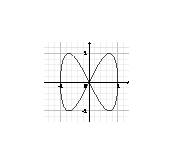
\includegraphics[width=2in]{Tut11-2b}
\end{center}
\end{enumerate}



 \item Find the length of the parametric curve:
\begin{enumerate}
 \item $x=-3\sin(2t)$, $y=3\cos(2t)$, $t\in [0,\pi]$.
 
 We have
 \[
 L = \int_0^{\pi}\sqrt{x'(t)^2+y'(t)^2}\,dt = \int_0^{\pi}\sqrt{36\cos^2(2t)+36\sin^2(2t)}\,dt = \int_0^{\pi}6\,dt = 6\pi.
 \]
 \item $x=e^{t/10}\cos t, y=e^{t/10}\sin t$, $t\in [0,2\pi]$.
 
 We first compute
 \begin{align*}
 x'(t) & = \frac{1}{10}e^{t/10}\cos(t)-e^{t/10}\sin(t)=e^{t/10}(\frac{1}{10}\cos(t)-\sin(t))\\
 y'(t) & = \frac{1}{10}e^{t/10}\sin(t)+e^{t/10}\cos(t)=e^{t/10}(\frac{1}{10}\sin(t)+\cos(t))\\
 x'(t)^2&= e^{2t/10}(\frac{1}{100}\cos^2(t)-\frac{2}{10}\cos(t)\sin(t)+\sin^2(t))\\
 y'(t)^2&= e^{2t/10}(\frac{1}{100}\sin^2(t)+\frac{2}{10}\cos(t)\sin(t)+\cos^2(t).
 \end{align*}
 Adding $x'(t)^2+y'(t)^2$, we see that the cross-terms cancel, and since $\sin^2(t)+\cos^2(t)=1$, we get
 \[
 \sqrt{x'(t)^2+y'(t)^2} = \sqrt{\frac{101}{100}e^{2t/10}}=\frac{\sqrt{101}}{10}e^{t/10}.
 \]
 Thus,
 \[
 L = \int_0^{2\pi}\sqrt{\frac{101}{100}}e^{t/10}\,dt = \sqrt{101}(e^{\pi/5}-1).
 \]
\end{enumerate}


 \item Find the area enclosed by the loop of the ``teardrop'' curve $x=t(t^2-1), y=t^2-1$. (See Figure 10.34 in the text.)

We first note that $x = t(t-1)(t+1)$, so $x=0$ for $t=0,1,-1$, while $y=0$ for $t=1, -1$. It follows (referring to the figure in the text) that the loop begins at $(0,0)$ when $t=-1$, and ends at $(0,0)$ when $t=1$. We check that $x>0$ for $-1<t<0$ and $x<0$ for $0<t<1$, which tells us that the loop is traversed in the clockwise direction. The area is thus given by
\begin{align*}
 A & = \int_{-1}^1 y\,dx = \int_{-1}^1 (t^2-1)(3t^2-1)\,dt \text{ (Note that $x(t)=t^3-t$, so $x'(t) = 3t^2-1$.)}\\
& = 2\int_0^1 (3t^4-4t^2+1)\,dt\\
& = 2\left(\frac{3}{5}-\frac{4}{3}+1\right) = \frac{8}{15}.
\end{align*}
 
 \textbf{Note:} For closed curves, it's always the case that the area is given by $\di\int_a^b y(t)x'(t)\,dt$ for clockwise orientation, and $\di-\int_a^by(t)x'(t)\,dt$ for counterclockwise orientation. Feel free to ask me if you want to know why it's not necessary to split the area up into pieces.
 
%\newpage

\item For each curve below, find the equation of the tangent line at the given value of $t$. Also: find all points where the tangent line is horizontal or vertical.
\begin{enumerate}
\item $x=t^2-1$, $y=t^3-t$, $t=1$.

The slope of the tangent line is
\[
m=\frac{dy}{dx}=\frac{y'(t)}{x'(t)} = \frac{3t^2-1}{2t}.
\]
When $t=1$ we get $x=0, y=0, m=1$, so our tangent line is $y=x$.

The tangent line is horizontal when $y'(t)=0$, so $t=\pm 1/\sqrt{3}$, and vertical when $x'(t)=0$, so $t=0$. 

(Additional care is required if $x'(t)$ and $y'(t)$ are simultaneously zero, but that's not the case here.)


\item $x=\cos(t), y=\sin(2t), t=\pi/4$

We have $\dfrac{dy}{dx} = \dfrac{y'(t)}{x'(t)} = -\dfrac{2\cos(2t)}{\sin(t)}$. When $t=\pi/4$ we have $x=1/\sqrt{2}$, $y=1$, and $m=0$, so our line is simply $y=1$.

The above is one horizontal tangent; we see that more generally $y'(t)=0$ when $t=\pi/4+k\pi/2$, where $k$ can be any integer.

We get a vertical tangent when $x'(t)=\sin(t)=0$, which occurs when $t=k\pi$, for any integer $k$.
\end{enumerate}
\end{enumerate}
\end{document}